\documentclass[letterpaper,11pt]{report}

\usepackage{fullpage}
\usepackage{verbatim}
\usepackage{cite}
\usepackage{setspace}
\usepackage{fancyhdr}

\usepackage[small]{caption}
\usepackage{graphics}
\usepackage{color}

\usepackage{hyperref}

\usepackage[dvips]{graphicx}
\graphicspath{ {images/} }

\usepackage{acro}

\setlength{\oddsidemargin}{-0.4mm} % 25 mm left margin
\setlength{\evensidemargin}{\oddsidemargin}
\setlength{\textwidth}{160mm}      % 25 mm right margin
\setlength{\topmargin}{-5.4mm}     % 20 mm top margin
\setlength{\headheight}{5mm}
\setlength{\headsep}{5mm}
\setlength{\footskip}{10mm}
\setlength{\textheight}{237mm}     % 20 mm bottom margin

\setlength{\parskip}{1ex}
\parindent 0in

\def\title{Building Management System : Scheduler and a web service to log data and control devices}

\acsetup{first-style=short}

\DeclareAcronym{ahu}{
  short = AHU ,
  long  = Air Handling Unit ,
  class = abbrev
}
\DeclareAcronym{api}{
  short = API ,
  long  = Application Program Interface ,
  class = abbrev
}
\DeclareAcronym{bms}{
  short = BMS ,
  long  = Building Management System ,
  class = abbrev
}
\DeclareAcronym{css}{
  short = CSS ,
  long  = Cascading Style Sheets ,
  class = abbrev
}
\DeclareAcronym{csu}{
  short = CSU ,
  long  = Ceiling Suspended Unit ,
  class = abbrev
}
\DeclareAcronym{dbms}{
  short = DBMS ,
  long  = Database Management System ,
  class = abbrev
}
\DeclareAcronym{fcu}{
  short = FCU ,
  long  = Fan Coil Unit ,
  class = abbrev
}
\DeclareAcronym{gui}{
  short = GUI ,
  long  = Graphical User Interface ,
  class = abbrev
}
\DeclareAcronym{html}{
  short = HTML ,
  long  = Hypertext Markup Language ,
  class = abbrev
}
\DeclareAcronym{http}{
  short = HTTP ,
  long  = Hypertext Transfer Protocol ,
  class = abbrev
}
\DeclareAcronym{hvac}{
  short = HVAC ,
  long  = Heating Ventilation and Air Conditioning ,
  class = abbrev
}
\DeclareAcronym{io}{
  short = I/O ,
  long  = Input/Output ,
  class = abbrev
}
\DeclareAcronym{lan}{
  short = LAN ,
  long  = Local Area Network ,
  class = abbrev
}
\DeclareAcronym{mac}{
  short = MAC ,
  long  = Media Access Control ,
  class = abbrev
}
\DeclareAcronym{os}{
  short = OS ,
  long  = Operating System ,
  class = abbrev
}
\DeclareAcronym{rest}{
  short = REST ,
  long  = Representational State Transfer ,
  class = abbrev
}
\DeclareAcronym{soc}{
  short = SoC ,
  long  = System on Chip ,
  class = abbrev
}
\DeclareAcronym{vfd}{
  short = VFD ,
  long  = Variable Frequency Drive ,
  class = abbrev
}
\DeclareAcronym{wifi}{
  short = WiFi ,
  long  = Wireless Fidelity ,
  class = abbrev
}

\begin{document}

\def\degreeone{B.Tech. in Computer Science and Engineering}
\def\degreetwo{B.Tech. in Electronics and Communication Engineering}
\def\btptrack{Engineering}
\def\submissiondate{November 17, 2016}
\def\supervisorone{Prof. Hemant Kumar}
\def\studentone{Divay Prakash, Amogh Vithalkar}
\def\rollnumberone{2014039, 2014134}
\def\titlelineone{Building Management System}
\def\titlelinetwo{Scheduler and a web service to log data and control devices}

\thispagestyle{empty}
\vspace{5.65in}

\begin{center}
\vspace{5.65in}
{\LARGE \bf \titlelineone{} : \titlelinetwo{}\\}
\vspace{.3in}
{\Large{Student Name: \studentone{}}}\\  
{\large{Roll Number: \rollnumberone{}}}\\
\vspace{.1in} 
\vspace{.65in}
\vspace{.65in}
{BTP report submitted in partial fulfillment of the requirements 
\\for the Degree of \degreeone{}/\\ \degreetwo{}\\}
on \submissiondate{}\\
\vspace{.65in}
\textbf{BTP Track}: \btptrack\\
\quad\\
{\textbf{BTP Advisor}\\ 
\supervisorone\\} 
\vspace{3.0in}
{Indraprastha Institute of Information Technology\\
New Delhi}
\end{center}


\newpage
\setcounter{page}{2}
\begin{center}
\textbf{\Large Student's Declaration}\label{section:declaration}
\end{center}
I hereby declare that the work presented in the report entitled \textbf{\title{}} submitted by me for the partial fulfillment of the requirements for the degree of \emph{Bachelor of Technology} in \emph{Computer Science \& Engineering} at Indraprastha Institute of Information Technology, Delhi, is an authentic record of my work carried out under guidance of \textbf{Prof. Hemant Kumar}. Due acknowledgements have  been given in the report to all material used. This work has not been submitted anywhere else for the reward of any other degree.\\
\vspace{0.5in}

\textbf{..............................}\hfill
\textbf{ Place \& Date: .............................}\\
\textbf{Divay Prakash}

\vspace{3in}
\begin{center}
\textbf{\Large Certificate} \label{section:certificate}
\end{center}
This is to certify that the above statement made by the candidate is correct to the best of my knowledge.\\
\vspace{0.4in}

\textbf{..............................}\hfill
\textbf{ Place \& Date: .............................}\\
\textbf{Prof. Hemant Kumar}

\pagebreak

\begin{abstract}
The building management HVAC(heating, ventilation and air conditioning) system for Phase II of IIIT-Delhi campus is designed to take care (and advantage) of diversity of use. Instead of using large AHUs(Air Handling Units), we will have individual units in faculty rooms, labs, and other spaces. This would allow us to condition air of the spaces that are occupied and the system would be able to maintain desired temperature more closely. The disadvantage of this approach is higher capital cost and a larger I/O points for BMS but the running cost will be saved. In this project we are developing a scheduler hosted on a web server to control the AC’s valves connected through Raspberry Pi and Arduino.
\par
\vspace{2.15in}
Keywords: building management system, scheduler, web server 
\end{abstract}

\newpage
\section*{Acknowledgments}\label{section:acknowledgments}
\pagestyle{plain}
\pagenumbering{roman}
I take this opportunity to express my deepest gratitude and appreciation to all those who have helped me directly or indirectly towards the successful completion of this project.
\par
I would like to express my sincere gratitude to my advisor Prof. Hemant Kumar for providing his invaluable guidance, comments and suggestions throughout the course of the project.

\newpage
\tableofcontents

\listoffigures
\addcontentsline{toc}{chapter}{List of Figures}

\newpage
\addcontentsline{toc}{chapter}{List of Abbreviations}
\chapter*{List of Abbreviations}
\printacronyms[include-classes=abbrev, heading=none]

\newpage
\chapter{Introduction}\label{chapter:introduction}
\pagenumbering{arabic}
\setcounter{page}{1}
\onehalfspacing
\section{BMS for phase I}
\ac{hvac} for the Phase I buildings (Academic, Lecture halls and library building) of IIIT-Delhi campus used large floor mounted \ac{ahu}'s to condition large spaces except lecture halls which were served by \ac{csu}'s (ceiling suspended units). Library building has one \ac{ahu} per floor feeding all the labs and rooms. The academic building has 6 AHUs (three serving A wing and the other three wing B). Hostels have one \ac{fcu} per room. The large AHUs of the academic block control volume of cold air by reducing the fan speed using \ac{vfd} drives. As the area per \ac{ahu} is large and the need very diverse (labs with varying number of occupants and equipment vs faculty rooms), the \ac{hvac} system is not very energy efficient and uniform temperature can't be maintained. The \ac{hvac} system has a very basic centralized control that can set temperature to be achieved in each one of the \ac{ahu}s or \ac{csu}s. It also allows switching on/ off, monitoring parameters etc centrally. Other than \ac{ahu}s/\ac{csu}s it can display status and parameters of chillers, cooling towers and hot water generator.
\par
In \ac{bms}/ \ac{hvac} terminology each point that is controlled or read is an \ac{io} point and an \ac{io} summary is prepared for any BMS installation to estimate the cost. The \ac{io} points are of 4 types - digital input, digital output, analog input and analog output. In phase I, we had chosen to only include \ac{io} that either needed to be controlled or the \ac{io} that were to be sensed and used for controlling to contain cost. The system was provided by Trane.
\par
Later a parallel system for monitoring and data collection was implemented by a research group led by Dr Amarjeet Singh. This group installed wireless temperature sensors (13) and Ethernet based power meters (500) all over the campus to optimize HVAC and energy use based on data collected.
\pagebreak
\section{\ac{bms} for phase II}
The \ac{hvac} for Phase II of IIIT-Delhi campus is designed to take care (and advantage) of diversity of use. So instead of large \ac{ahu}s, we will have individual units in faculty rooms, labs, and other spaces. This would allow us to condition air of the spaces that are occupied and the system would be able to maintain desired temperature more closely. The disadvantage of this approach is higher capital cost and a larger \ac{io} points for \ac{bms} but the running cost will be saved.

\newpage
\chapter{Problem Statement}\label{chapter:problemstatement}
\onehalfspacing
Given the large number of units to monitor and control, the cost of \ac{bms} was estimated to be very high. In addition, for phase II, the traditional system would be close-ended and proprietary.
\par
Most of the cost (about 60\%) would have been in the wiring the large number of units to controllers. This cost can be saved if individual \ac{wifi}-based controllers (500-600) were to be deployed. These wireless devices can use the existing institute \ac{lan} infrastructure to further save costs. In addition, groups of these devices would be controlled by Raspberry Pi devices running a custom Django server which would further be controlled by a central Django server. This central server would provide a \ac{gui} for administrators to monitor and control the entire \ac{bms} system.

\newpage
\chapter{Architecture}\label{chapter:architecture}
\onehalfspacing
\begin{figure}[h]
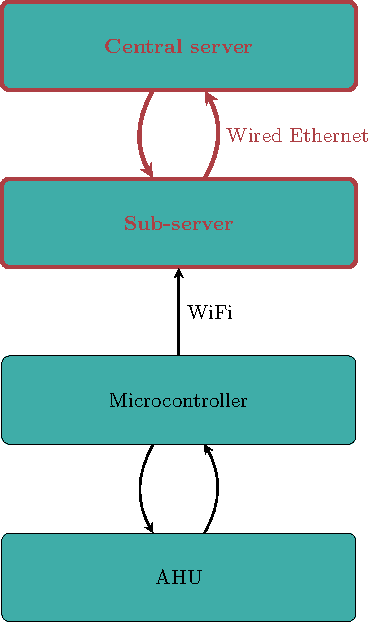
\includegraphics[width=14cm, height=10cm]{arch}
\centering
\captionsetup{justification=centering}
\caption{Block diagram of the building management system project}
\label{fig:arch}
\end{figure}
The \ac{bms}/ \ac{hvac} system, is structured in the manner described by figure \ref{fig:arch}. At the lowest level is the \ac{ahu}, which performs the actual cooling/heating functionality of the system. It is controlled by the microcontroller. The microcontroller monitors various system parameters and accordingly runs the \ac{ahu}. The microcontroller runs in a master-slave configuration wherein the master is an ESP8266 wireless module which is responsible for communication with further control levels. This system is in controlled by a Raspberry Pi sub-server unit, which is responsible for logging data and passing control instructions to the microcontroller/wifi module unit according to policies set by the central server. The highlighted sections in figure \ref{fig:arch} are the modules that were worked upon over the course of this project.

\newpage
\chapter{Design}\label{chapter:Design}
\onehalfspacing
\section{Overview}
\begin{figure}[h]
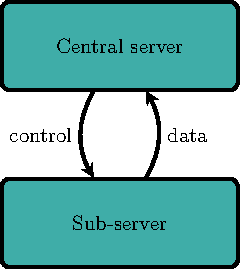
\includegraphics[width=4cm, height=4.5cm]{des}
\centering
\captionsetup{justification=centering}
\caption{Higher level control modules of the building management system}
\label{fig:des}
\end{figure}
The higher level control of the building management system is carried out by the central server in conjunction with various sub-server units managing their own group of microcontroller devices. The details of the central server and the sub-servers are given in the following sections.
\section{Central server}
The central server of the system is a software implementation only. There are no specific hardware requirements for the same. The server is implemented in such a manner so as to be able to provide interfaces to both the sub-server devices using a \ac{rest} \ac{api} and also to system administrators by way of a \ac{gui}. If required, the central server could be on the cloud. The server can be broken down into two main modules, the frontend and the backend. Both of these modules were built over the course of this project.
\subsection{Design specifications}
\subsubsection{Frontend}
The frontend of the central server consists of a hierarchy of web pages created using \ac{html}/\newline \ac{css}/JavaScript/jQuery and the Bootstrap framework. This provides the \ac{gui} which can be used by system administrators for overall analysis/control of the system.
\subsubsection{Backend}
The backend of the central server consists of a web application created using the Python web framework Django. The system uses time series database for storing the client data.
\subsection{Design choices}
There are various design choices that had to be made in order to create a cohesive and well-structured central server for the \ac{bms} project. The central server is implemented as a web application. The choice of a web-application was made keeping in mind the advantages of web applications over traditional desktop applications -
\begin{itemize}
    \item Easier deployment - The application does not need to be individually deployed to any client machine. The client machine only requires a functioning web browser to access the system.
    \item Maintenance - System maintenance is vastly easier as all updates and bug fixes need to be introduced at the server end only. In the same manner, regular updates are also easy.
    \item Platform independent - This was the major reason in favour of using a web application. The server implemented as a web application provides complete functionality to clients running any \ac{os}.
    \item Faster development process - By using a web application, users access the system by way of a web browser. This creates a uniform environment across platforms. While user interaction with the application needs to be thoroughly tested on different web browsers, the application itself needs only be developed for a single operating system. There is no need to develop and test it on all possible operating system versions and configurations. This makes development and troubleshooting much easier.
    \item Scalability - Being independent of hardware configurations, web applications are easily scalable. It is possible to scale the system with growing \ac{io} points or number of client instances.
\end{itemize}
\section{Sub-server}
\subsection{Design specifications}
The sub-servers are individual Raspberry Pi units running a Linux \ac{os} distribution. These devices are connected to the central server using a wired Ethernet connection and each unit manages up to 20 AVR microcontroller units over a \ac{wifi} interface. The Raspberry Pi devices host a web server which provides various functionalities.
\subsection{Design choices}
The choice of using a Raspberry Pi device for the sub-server was made considering the following points -
\begin{itemize}
    \item Ease of deployment - Due to the small size of the device, it is easy to deploy unobtrusively in extremely small spaces such as wiring closets and channels, where power supply and Ethernet cables are available.
    \item \ac{soc} - The Raspberry Pi provides us a complete system on chip ie. it integrates all the components of a computer on one single chip. This micro-computer does not require any additional chips for its functionality, with a built-in Ethernet interface.
\end{itemize}

\newpage
\chapter{Implementation}\label{chapter:Implementation}
\onehalfspacing
\section{Central server}
\subsection{Description}
The central server is a Django web application which uses a time-series \ac{dbms}. The frontend part of the web application is done using \ac{html}/\ac{css} and bootstrap.
\subsection{Functionality}
The central server has been coded as a stand-in for a more comprehensive implementation in the future. Presently, it consists of a barebones Django server with little functionality apart from receiving data files from  and sending configuration files to the sub-server units.
\section{Sub-server}
\subsection{Description}
The Raspberry Pi units serving as sub-servers run a Django based web application which serves a \ac{rest} \ac{api}. This is utilised by both the ESP devices and the central server which communicate with the device using \ac{http} messages. This is further explained in the next section. Over the course of this project, the entire Django server was rewritten to provide enhanced functionality while being lightweight. The database system being used to store client data was moved from a MySQL database management system to a flat file system.
\subsection{Functionality}
\subsubsection{For ESP device}
Communication taking place between sub-server devices and the ESP devices follows the client-server model in case of data logging, whereas in the case of setting configuration, the sub-server (Rapberry Pi device) initiates a message to the client (ESP device) without a prior request from the client.
\begin{itemize}
    \item Data logging - The sub-server device provides a \ac{rest} \ac{api} method for ESP devices to log data. The ESP device makes an \ac{http} POST request to the Raspberry Pi sub-server, which processes the attached data and stores it in a file. This data is stored using the ESP \ac{mac} addresses and the \ac{http} sub-server timestamp as keys. Thereafter, the sub-server sends a confirmation message back to the client.
    \item Setting configuration - The ESP devices also receives configuration messages from the sub-server units. These messages contain the register values which will be written to the microcontroller for \ac{ahu} control.\hfill \break The sub-server extracts the ESP devices' \ac{mac} address from the configuration file, along with the data to be sent to the client. It then makes an \ac{http} GET request to the ESP device containing the data.
\end{itemize}
\subsubsection{For central server}
\begin{itemize}
    \item Receive configuration file - The sub-server device acts as a client for this method, used by the central server to transmit a \verb|json| file to the sub-server using an \ac{http} POST message.
    \item Send logging data - The Raspberry Pi device sends the data log to the central server using \ac{http} POST message containing a log file at a fixed time interval. This enables the deletion of the files at sub-server end, freeing up valuable memory resources.
\end{itemize}

\newpage
\nocite*{}
\bibliographystyle{acm}
\addcontentsline{toc}{chapter}{Bibliography}
\bibliography{bibdb}

\end{document}
